\section{ALICE Computing model}

In this section, we will briefly describe the computing model of the
ALICE experiment \cite{ALICETDR}.

ALICE (A Large Ion Collider Experiment) is a dedicated heavy-ion
(HI) experiment at the CERN LHC which apart from the HI mission has
also its proton-proton (pp) Physics program. Together with the other
LHC experiments, ALICE has been successfully taking and processing
pp and HI data since the LHC startup in November 2009. During the pp
running, the data taking rate has been up to 500 MB/s while during
the HI running the data was taken with the rate up to 2.5 GB/s. As
already mentioned, during 2010 the total volume of data taken by
all the LHC experiments reached 15~PB, which corresponds to 7~months
of the pp running and 1 month of the HI running (together with
4~months of an LHC technical stop for maintenance and upgrades this
makes up for one standard data taking year (SDTY)).

The computing model of ALICE relies on the ALICE Computing Grid, the
distributed computing infrastructure based on the hierarchical Tier
structure as described in section 2.  ALICE has developed over the
last 10 years a distributed computing environment and its
implementation: the Grid middleware suite AliEn (AliCE Environment)
[26], which is integrated in the WLCG environment. It provides a
transparent access to computing resources for the ALICE community
and will be described in the next section.

\subsection{Raw data taking, transfer and registration}
%
The ALICE detector consists of 18~subdetectors that interact with
5~online systems. During data taking, the data is read out by
the Data Acquisition (DAQ) system as raw data streams produced by
the subdetectors, and is moved and stored over several media. On
this way, the raw data is formatted, the events (data sets
containing information about individual pp or Pb-Pb collisions) are
built, the data is objectified in the ROOT format and then
recorded on a local disk. During the intervals of continuous data
taking called runs, different types of data sets can be collected of
which the so-called PHYSICS runs are those substantial for Physics
analysis. There are also all kinds of calibration and other
subdetectors' testing runs important for the reliable subsystems
operation.

ALICE experimental area (called Point2 (P2)) serves as an
intermediate storage: the final destination of the collected raw
data is the CERN Advanced STORage system (CASTOR) , the permanent
data storage (PDS) at the CERN Computing center. From Point2, the
raw data is transferred to the disk buffer adjacent to CASTOR at
CERN (see Figure~\ref{fig11}). As mentioned before, the transfer
rates are up to 500 MB/s for the pp and up to 2.5 GB/s for the HI
data taking periods.

%fig11
\begin{figure}[htb] % h-here, t-top, b-bottom
\centering
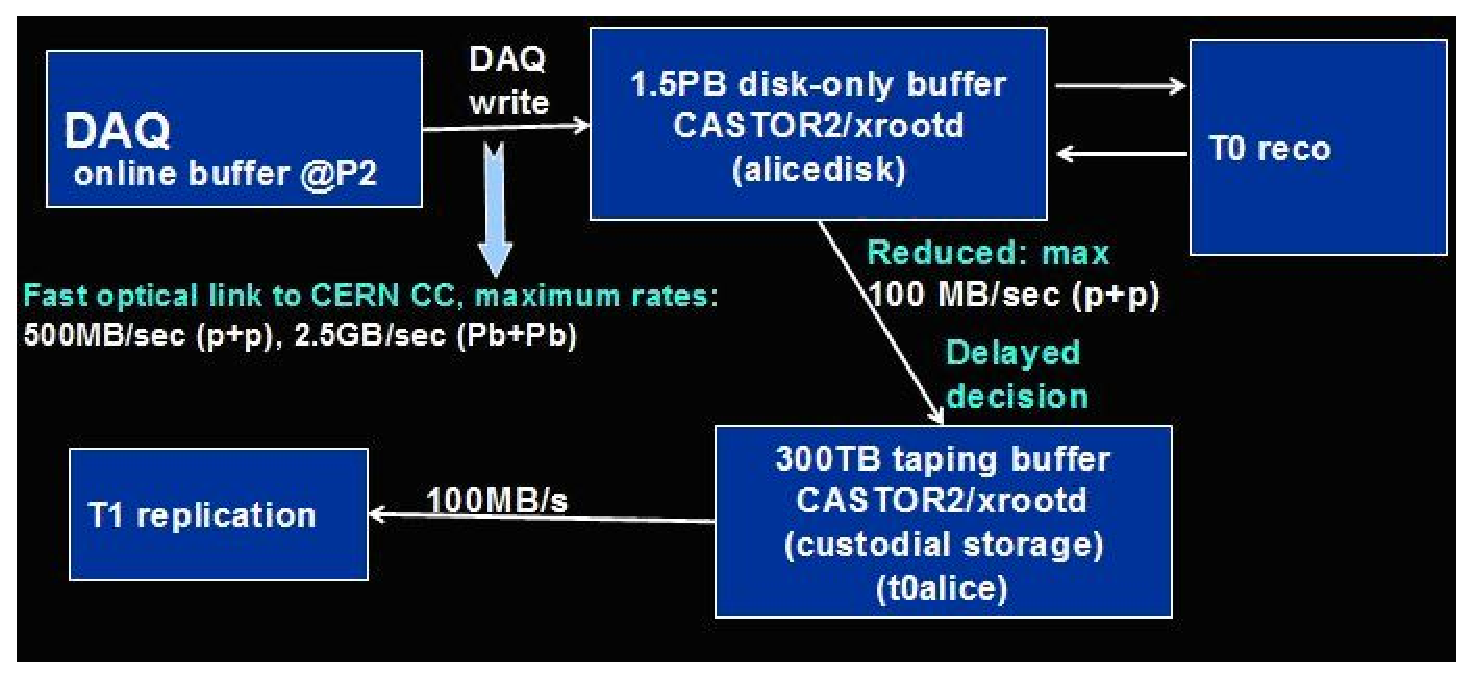
\includegraphics[width=13cm]{fig11.eps} %    ** if .eps don't need extension
\caption{Data processing chain}\label{fig11}
\end{figure}



After the migration to the CERN Tier-0, the raw data is registered
in the AliEn catalogue [26] and the data from PHYSICS runs is
automatically queued for the Pass1 of reconstruction, the first part
of the data processing chain, which is performed at the CERN Tier-0.
In parallel with the reconstrucion, the data from PHYSICS runs is also
automatically queued for the replication to external Tier-1s (see
Figure~\ref{fig11}). It may happen that the replication is launched
and finished fast and the data goes through the first processing at
a Tier-1.

The mentioned automated processes are a part of a complex set of
services deployed over the ALICE Computing Grid infrastructure. All
the involved services are continuously controlled by automatic
procedures, reducing to a minimum the human interaction. The Grid
monitoring environment adopted and developed by ALICE, the
Java-based MonALISA (MONitoring Agents using Large Integrated
Services Architecture) \cite{MonALISA}, uses decision-taking automated agents
for management and control of the Grid services. For monitoring of
raw data reconstruction passes see \cite{ALICE_PROD}.

The automatic reconstruction is typically completed within a couple
of hours after the end of the run. The output files from the
reconstruction are registered in AliEn and are available on the Grid
(stored and accessible within the ALICE distributed storage pool)
for further processing.

\subsection{AliRoot}
%
AliRoot \cite{AliRoot} is the ALICE software framework for reconstruction, simulation and
analysis of the data. It has been under a steady
development since 1998. Typical use cases include detector
description, events generation, particle transport, generation of
``summable digits'', event merging, reconstruction, particle
identification and all kinds of analysis tasks. AliRoot uses the
ROOT system as a foundation on which the framework is built. The Geant3 \cite{GEANT3} or
FLUKA \cite{FLUKA} packages perform the transport of particles through the
detector and simulate the energy deposition from which the detector
response can be simulated. Except for large existing libraries, such
as Pythia6 \cite{pythia} and HIJING \cite{hijing}, and some remaining legacy code,
this framework is based on the Object Oriented programming paradigm
and is written in C++.

AliRoot is constituted by a large amount of files, sources,
binaries, data and related documentation. Clear and efficient
management guidelines are vital if this corpus of software should
serve its purpose along the lifetime of the ALICE experiment. The
corresponding policies are described in \cite{ALICE_POLICY}.  For understanding and
improvement of the AliRoot performance, as well as for understanding
the behavior of the ALICE detectors, the fast feedback given by the
offline reconstruction is essential.

\subsection{Multiple reconstruction}
%
In general, the ALICE computing model for the pp data taking is
similar to that of the other LHC experiments. Data is automatically
recorded and then reconstructed quasi online at the CERN Tier-0
facility. In parallel, data is exported to the different external
Tier-1s, to provide two copies of the raw data, one stored at the
CERN CASTOR and another copy shared by all the external Tier-1s.

For HI (Pb-Pb) data taking this model is not viable, as data is
recorded at up to 2.5~GB/s.  Such a massive data stream would
require a prohibitive amount of resources for quasi real-time
processing. The computing model therefore requires that the HI data
reconstruction at the CERN Tier-0 and its replication to the Tier-1s
be delayed and scheduled for the period of four months of the LHC
technical stop and only a small part of the raw data (10-15\%) be
reconstructed for the quality checking. In reality, comparatively
large part of the HI data (about 80\%) got reconstructed and
replicated in 2010 before the end of the data taking due to
occasional lapses in the LHC operations and much higher quality of
the network infrastructure than originally envisaged.

After the first pass of the reconstruction, the data is usually
reconstructed subsequently more times (up to 6-7 times) for better
results at Tier-1s or Tier-2s . Each pass of the reconstruction
triggers a cascade of additional tasks organized centrally like
Quality Assurance (QA) processing trains and a series of different
kinds of analysis trains described later. Also, each reconstruction
pass triggers a series of the Monte Carlo simulation productions.
All this complex of tasks for a given reconstruction pass is
launched automatically as mentioned before.

\subsection{Analysis}
%
The next step in the data processing chain is then the analysis.
There are two types of analysis: a scheduled analysis organized
centrally and then the end-user, so-called chaotic analysis. Since
processing of the end-user analysis jobs often brings some problems
like a high memory consumption (see Figure~\ref{fig12}) or unstable
code, the scheduled analysis is organized in the form of so called
analysis trains \cite{trains}. The trains absorb up to 30 different
analysis tasks running in succession with one data set read and with
a very well controlled environment. This helps to consolidate the
end-user analysis.

%fig12
\begin{figure}[htb] % h-here, t-top, b-bottom
\centering
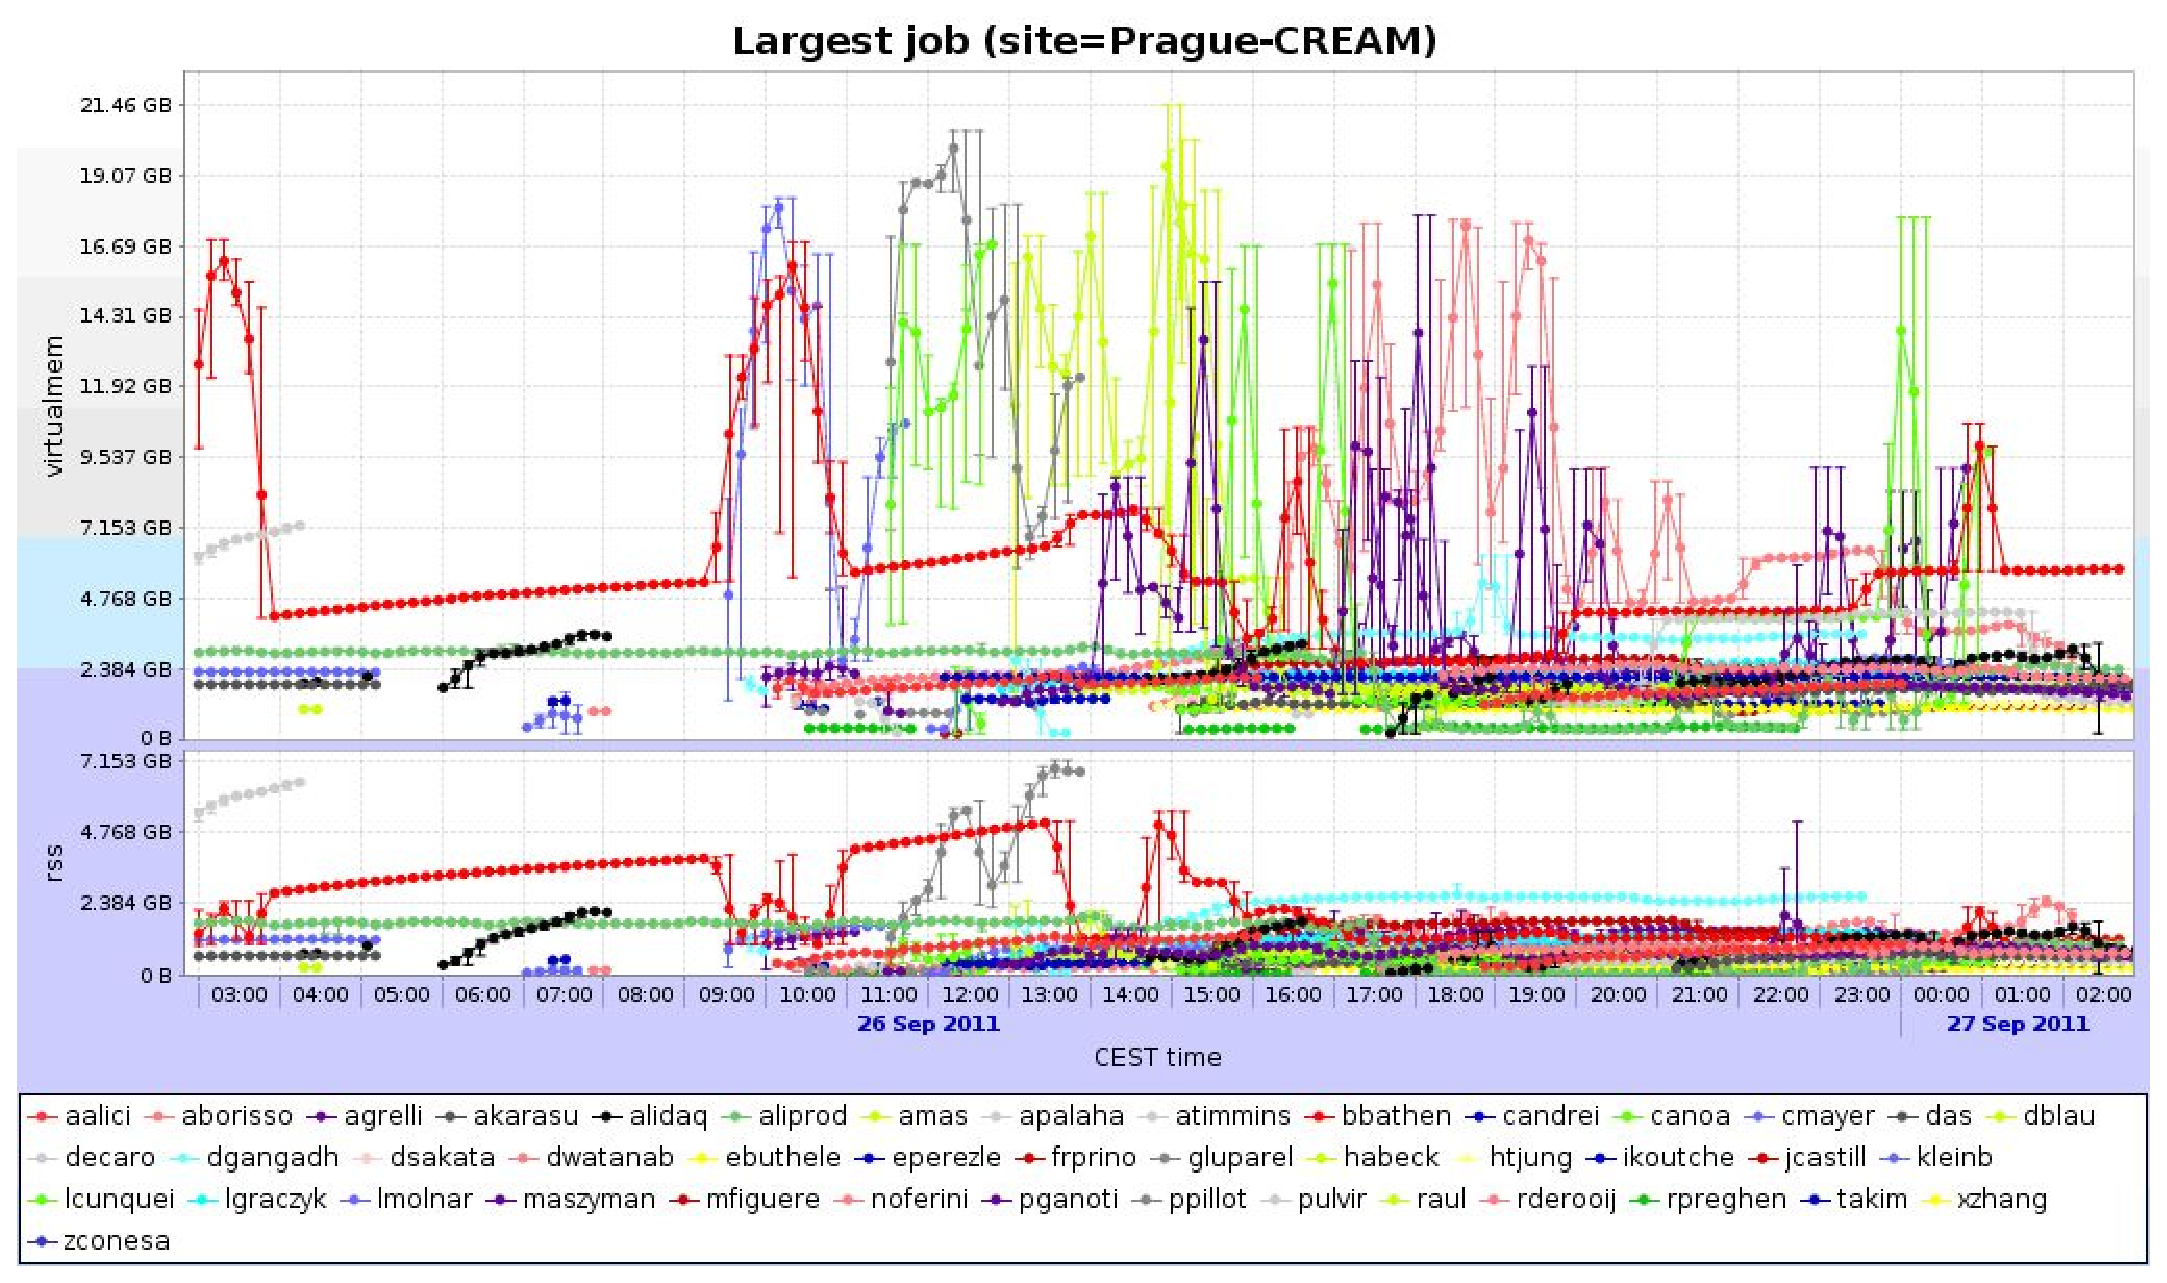
\includegraphics[width=13cm]{fig12.eps} %    ** if .eps don't need extension
\caption{End-user analysis memory consumption: peaks in excess of
20~GB}\label{fig12}
\end{figure}


The computing model assumes that the scheduled analysis will be
performed at Tier-1 sites, while the chaotic analysis and simulation
jobs will be performed at Tier-2s. The experience gained during the
numerous Data Challenges, the excellent network performance, the
stable and mature Grid middleware deployed over all sites and the
conditions at the time of the real data taking in 2010/2011
progressively replaced the original hierarchical scenario by a more
``symmetric'' model often referred to as the ``cloud model''.

\subsection{Simulations}
%
As already mentioned, ever since the start of building the ALICE
distributed computing infrastructure, the system was tested and
validated with increasingly massive productions  of Monte Carlo (MC)
simulated events of the LHC collisions in the ALICE detector. The
simulation framework \cite{simulation} covers the simulation of primary collisions
and generation of the emerging particles, the transport of particles
through the detector, the simulation of energy depositions (hits) in
the detector components, their response in form of so called
summable digits, the generation of digits from summable digits with
the optional merging of underlying events and the creation of raw
data. Each raw data production cycle triggers a series of
corresponding MC productions \cite{mc}. As a result, the volume of
data produced during the MC cycles is usually in excess of the
volume of the corresponding raw data.

\subsection{Data types}
%
To complete the description of the ALICE data processing chain, we
will mention the different types of data files produced at different
stages of the chain (see Figure~\ref{fig13}).

As was already mentioned, the data is delivered by the Data
Acquisition system in a form of raw data in the ROOT format. The
reconstruction produces the so-called Event Summary Data (ESD), the
primary container after the reconstruction. The ESDs contain
information like run and event numbers, trigger class, primary
vertex, arrays of tracks/vertices, detector conditions. In an ideal
situation following the computing model, the EODs should be of 10\%
size of the corresponding raw data files.

The subsequent data processing provides so called Analysis Object
Data (AOD), the secondary processing product, which are data objects
containing more skimmed information needed for final analysis.
According to the Computing model, the size of AODs should be 2\% of
the raw data file size. Since it is difficult to squeeze all the
information needed for the Physics results in such small data
containers, this limit was not yet fully achieved.

%fig13
\begin{figure}[htb] % h-here, t-top, b-bottom
\centering
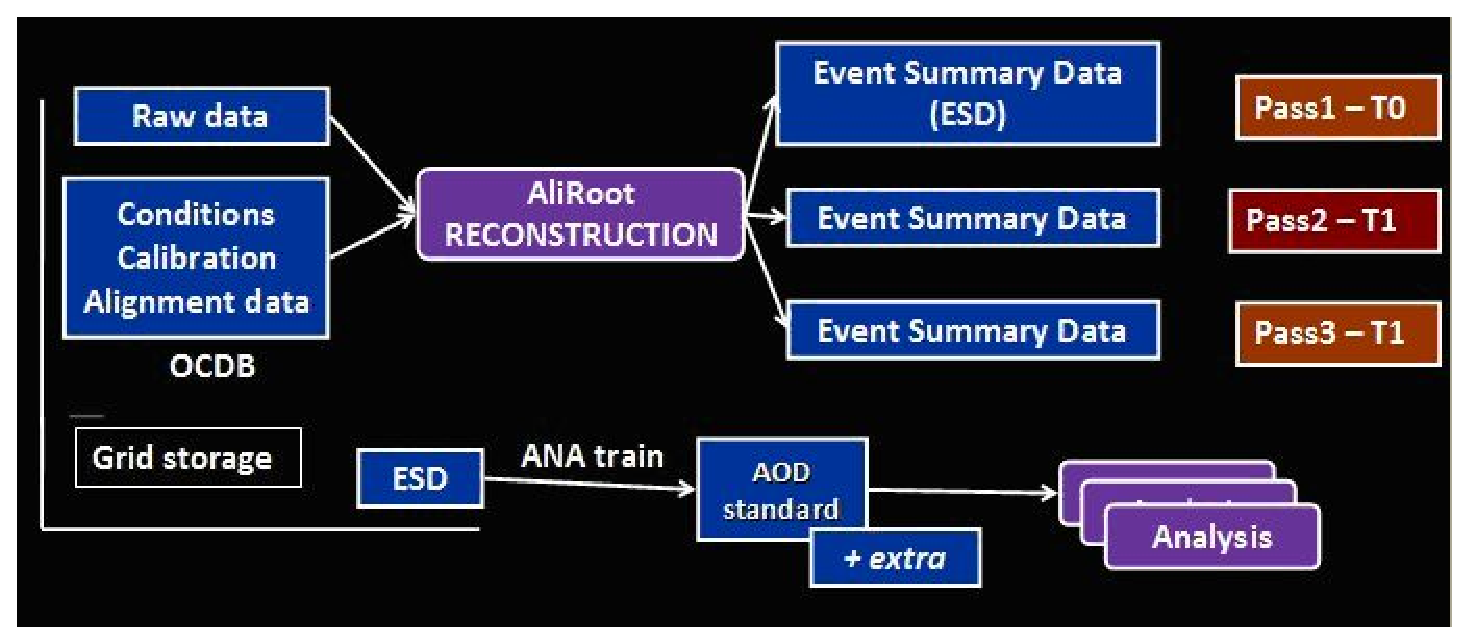
\includegraphics[width=13cm]{fig13.eps} %    ** if .eps don't need extension
\caption{Data types produced in the processing chain}\label{fig13}
\end{figure}


\subsection{Resources}
%
The ALICE distributed computing infrastructure has evolved from a
set of about 20 computing sites into a global world-wide system of
distributed resources for data storage and processing. As of today,
this project is made of over 80 sites spanning 5 continents (Africa,
Asia, Europe, North and South America), involving 6 Tier-1 centers
and more than 70 Tier-2 centers \cite{sites}, see also Figure~\ref{fig14}.
Altogether, the resources provided by the ALICE sites represent in
excess of 20 thousands of CPUs, 12~PB of distributed disk storage
and 30~PB of distributed tape storage, and the gradual upscale of
this capacity is ongoing.  Similar to other LHC experiments, about
half of the CPU and disk resources is provided by the Tier-2
centers. For the year 2012, ALICE plans/requirements for computing
resources within WLCG represent 211.7 of kHEP-SPEC06 CPU capacity,
38.8~PB of disk storage and 36.6~PB of tapes\cite{resources}.

%fig14
\begin{figure}[htb] % h-here, t-top, b-bottom
\centering
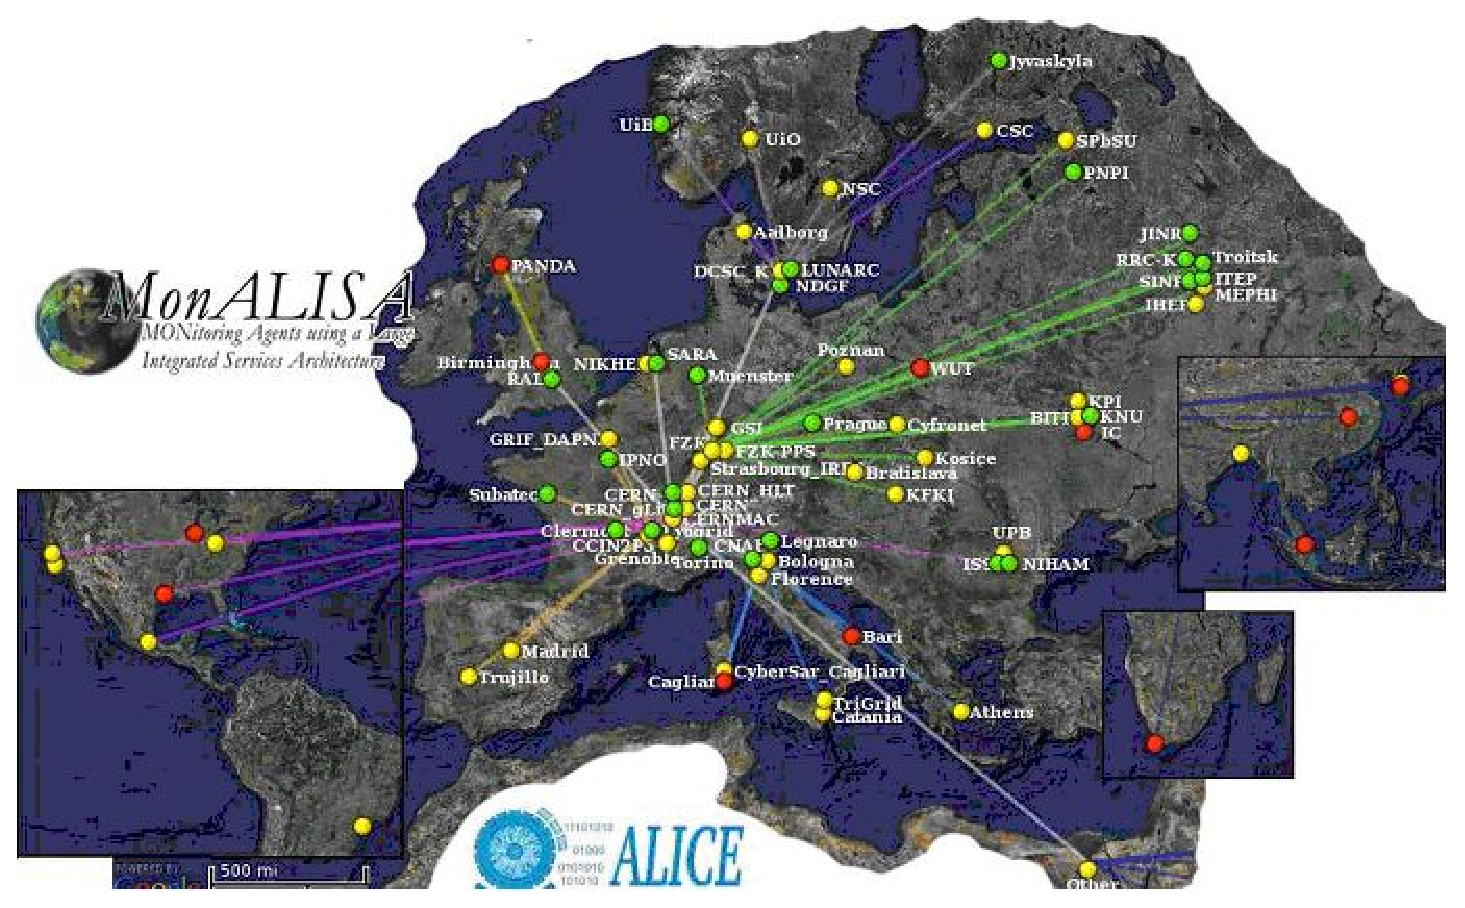
\includegraphics[width=13cm]{fig14.eps} %    ** if .eps don't need extension
\caption{ALICE sites}\label{fig14}
\end{figure}


\subsection{Concluding remarks}
%
The concept of the ALICE computing model was officially proposed in
2005. Since then, it has been used for massive Monte Carlo event
productions, for end-user analysis and for the raw data management
and processing. The strategy has been validated under heavy load
during a series of Data Challenges and during the real data taking
in 2010/2011. The model provides the required Grid functionality via
a combination of the common Grid services offered on the WLCG
resources and the ALICE-specific services from AliEn. Today's
computing environments are anything but static. Fast development in
Information Technologies, commodity hardware (hardware being
constantly replaced and operating systems upgraded), Grid software
and networking technologies inevitably boosted also further
development of the ALICE computing model. One of the main effects is
a transformation of the model from the strictly hierarchical
Tier-like structure to a more loose scenario, a ``cloud-like''
solution.
